% Options for packages loaded elsewhere
% Options for packages loaded elsewhere
\PassOptionsToPackage{unicode}{hyperref}
\PassOptionsToPackage{hyphens}{url}
%
\documentclass[
  10pt,
  ignorenonframetext,
  aspectratio=169,
  spanish,
]{beamer}
\newif\ifbibliography
\usepackage{pgfpages}
\setbeamertemplate{caption}[numbered]
\setbeamertemplate{caption label separator}{: }
\setbeamercolor{caption name}{fg=normal text.fg}
\beamertemplatenavigationsymbolshorizontal
% remove section numbering
\setbeamertemplate{part page}{
  \centering
  \begin{beamercolorbox}[sep=16pt,center]{part title}
    \usebeamerfont{part title}\insertpart\par
  \end{beamercolorbox}
}
\setbeamertemplate{section page}{
  \centering
  \begin{beamercolorbox}[sep=12pt,center]{section title}
    \usebeamerfont{section title}\insertsection\par
  \end{beamercolorbox}
}
\setbeamertemplate{subsection page}{
  \centering
  \begin{beamercolorbox}[sep=8pt,center]{subsection title}
    \usebeamerfont{subsection title}\insertsubsection\par
  \end{beamercolorbox}
}
% Prevent slide breaks in the middle of a paragraph
\widowpenalties 1 10000
\raggedbottom
\AtBeginPart{
  \frame{\partpage}
}
\AtBeginSection{
  \ifbibliography
  \else
    \frame{\sectionpage}
  \fi
}
\AtBeginSubsection{
  \frame{\subsectionpage}
}
\usepackage{iftex}
\ifPDFTeX
  \usepackage[T1]{fontenc}
  \usepackage[utf8]{inputenc}
  \usepackage{textcomp} % provide euro and other symbols
\else % if luatex or xetex
  \usepackage{unicode-math} % this also loads fontspec
  \defaultfontfeatures{Scale=MatchLowercase}
  \defaultfontfeatures[\rmfamily]{Ligatures=TeX,Scale=1}
\fi
\usepackage{lmodern}

\usetheme[]{Madrid}
\ifPDFTeX\else
  % xetex/luatex font selection
\fi
% Use upquote if available, for straight quotes in verbatim environments
\IfFileExists{upquote.sty}{\usepackage{upquote}}{}
\IfFileExists{microtype.sty}{% use microtype if available
  \usepackage[]{microtype}
  \UseMicrotypeSet[protrusion]{basicmath} % disable protrusion for tt fonts
}{}
\makeatletter
\@ifundefined{KOMAClassName}{% if non-KOMA class
  \IfFileExists{parskip.sty}{%
    \usepackage{parskip}
  }{% else
    \setlength{\parindent}{0pt}
    \setlength{\parskip}{6pt plus 2pt minus 1pt}}
}{% if KOMA class
  \KOMAoptions{parskip=half}}
\makeatother


\usepackage{longtable,booktabs,array}
\newcounter{none} % for unnumbered tables
\usepackage{calc} % for calculating minipage widths
\usepackage{caption}
% Make caption package work with longtable
\makeatletter
\def\fnum@table{\tablename~\thetable}
\makeatother
\usepackage{graphicx}
\makeatletter
\newsavebox\pandoc@box
\newcommand*\pandocbounded[1]{% scales image to fit in text height/width
  \sbox\pandoc@box{#1}%
  \Gscale@div\@tempa{\textheight}{\dimexpr\ht\pandoc@box+\dp\pandoc@box\relax}%
  \Gscale@div\@tempb{\linewidth}{\wd\pandoc@box}%
  \ifdim\@tempb\p@<\@tempa\p@\let\@tempa\@tempb\fi% select the smaller of both
  \ifdim\@tempa\p@<\p@\scalebox{\@tempa}{\usebox\pandoc@box}%
  \else\usebox{\pandoc@box}%
  \fi%
}
% Set default figure placement to htbp
\def\fps@figure{htbp}
\makeatother



\ifLuaTeX
\usepackage[bidi=basic,shorthands=off]{babel}
\else
\usepackage[bidi=default,shorthands=off]{babel}
\fi
\ifLuaTeX
  \usepackage{selnolig} % disable illegal ligatures
\fi


\setlength{\emergencystretch}{3em} % prevent overfull lines

\providecommand{\tightlist}{%
  \setlength{\itemsep}{0pt}\setlength{\parskip}{0pt}}



 


% Color rojo vino / Burgundy
\definecolor{RojoVino}{HTML}{722F37}
\definecolor{burgundy}{RGB}{128, 0, 32}
\definecolor{darkwine}{RGB}{90, 0, 20}
\definecolor{softwine}{RGB}{250, 240, 242}
\definecolor{charcoal}{RGB}{40, 40, 40}

% Configuración de colores Beamer
\setbeamercolor{structure}{fg=RojoVino}
\setbeamercolor{palette primary}{bg=RojoVino,fg=white}
\setbeamercolor{palette secondary}{bg=RojoVino!85!black,fg=white}
\setbeamercolor{palette tertiary}{bg=RojoVino!70!black,fg=white}

% Pie de página
\setbeamercolor{author in head/foot}{bg=RojoVino, fg=white}
\setbeamercolor{title in head/foot}{bg=RojoVino!90!black, fg=white}
\setbeamercolor{date in head/foot}{bg=RojoVino!80!black, fg=white}

% Estilo de bloques
\setbeamercolor{block title}{bg=RojoVino,fg=white}
\setbeamercolor{block body}{bg=softwine,fg=black}

% Logo dinámico (diapositivas > 1)
\logo{%
  \ifnum\insertframenumber>1%
    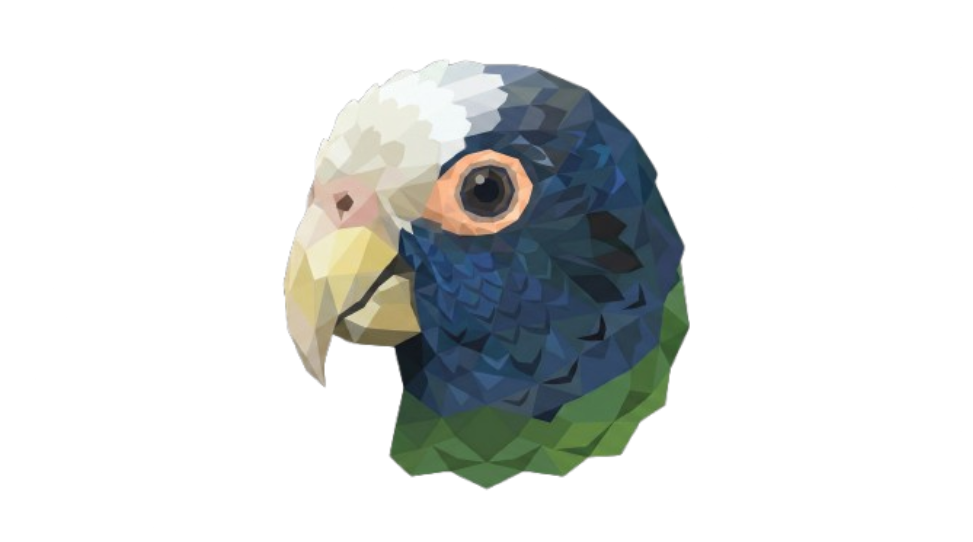
\includegraphics[height=0.8cm]{bonita.png}%
  \fi%
}

% Logo grande en la portada
\titlegraphic{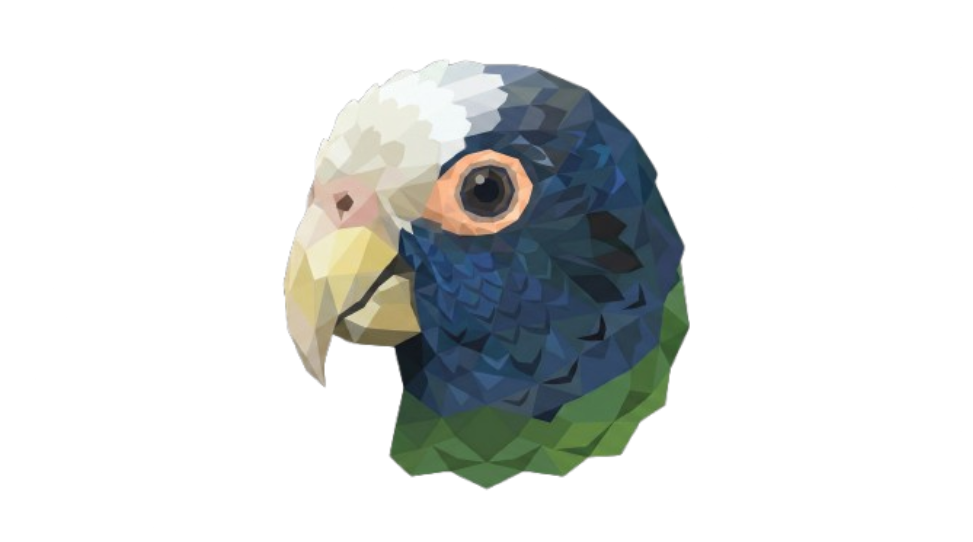
\includegraphics[height=2.5cm]{bonita.png}}

% Opciones estéticas generales
\setbeamertemplate{blocks}[rounded][shadow=false]
\setbeamertemplate{navigation symbols}{}
\setbeamertemplate{caption}[numbered]
\setbeamerfont{caption name}{series=\bfseries}
\makeatletter
\@ifpackageloaded{caption}{}{\usepackage{caption}}
\AtBeginDocument{%
\ifdefined\contentsname
  \renewcommand*\contentsname{Tabla de contenidos}
\else
  \newcommand\contentsname{Tabla de contenidos}
\fi
\ifdefined\listfigurename
  \renewcommand*\listfigurename{Listado de Figuras}
\else
  \newcommand\listfigurename{Listado de Figuras}
\fi
\ifdefined\listtablename
  \renewcommand*\listtablename{Listado de Tablas}
\else
  \newcommand\listtablename{Listado de Tablas}
\fi
\ifdefined\figurename
  \renewcommand*\figurename{Figura}
\else
  \newcommand\figurename{Figura}
\fi
\ifdefined\tablename
  \renewcommand*\tablename{Tabla}
\else
  \newcommand\tablename{Tabla}
\fi
}
\@ifpackageloaded{float}{}{\usepackage{float}}
\floatstyle{ruled}
\@ifundefined{c@chapter}{\newfloat{codelisting}{h}{lop}}{\newfloat{codelisting}{h}{lop}[chapter]}
\floatname{codelisting}{Listado}
\newcommand*\listoflistings{\listof{codelisting}{Listado de Listados}}
\makeatother
\makeatletter
\makeatother
\makeatletter
\@ifpackageloaded{caption}{}{\usepackage{caption}}
\@ifpackageloaded{subcaption}{}{\usepackage{subcaption}}
\makeatother

\usepackage{bookmark}
\IfFileExists{xurl.sty}{\usepackage{xurl}}{} % add URL line breaks if available
\urlstyle{same}
\hypersetup{
  pdftitle={Remesas{,} Índice de Tipo de Cambio Real y Competitividad},
  pdfauthor={Emerson Lopez},
  pdflang={es},
  hidelinks,
  pdfcreator={LaTeX via pandoc}}


\title{\texorpdfstring{Remesas, Índice de Tipo de Cambio Real y
Competitividad}{Remesas{,} Índice de Tipo de Cambio Real y Competitividad}}
\subtitle{\texorpdfstring{Un enfoque BVECM para Nicaragua
(2006--2023)}{Un enfoque BVECM para Nicaragua (2006--2023)}}
\author{Emerson Lopez}
\date{13 de agosto de 2026}
\institute{Universidad Nacional de Ingeniería (UNI)}

\begin{document}
\frame{\titlepage}


\begin{frame}{Comienzo y Retos}
\protect\phantomsection\label{comienzo-y-retos}
\begin{itemize}
\tightlist
\item
  \textbf{Origen:} Practica econometría con datos reales.
\item
  \textbf{Intentos:} Regresiones OLS normales cruzando el PIB, las
  remesas y otras variables.
\item
  \textbf{Fenómeno:} El auge de las remesas en 2024 era exponencial.
\item
  \textbf{Investigación:} Enfermedad Holandesa.
\end{itemize}

\begin{block}{Programación}
\protect\phantomsection\label{programaciuxf3n}
RStudio, documentación de las librerías, funciones y vídeos tutoriales.
\end{block}

\vspace{0.3cm}

\begin{block}{Metodológica}
\protect\phantomsection\label{metodoluxf3gica}
Los modelo OLS era demasiado básico para capturar la dinámica real de
estas variables.
\end{block}
\end{frame}

\begin{frame}{Datos}
\protect\phantomsection\label{datos}
La limpieza y transformación de datos:

\begin{itemize}
\tightlist
\item
  \textbf{El problema del tamaño muestral bajo:}

  \begin{itemize}
  \tightlist
  \item
    \emph{Anual (2006--2023):} Solo 17 observaciones.
  \item
    \emph{Trimestral:} Eran más observaciones, pero seguían siendo
    bajas.
  \item
    \emph{Mensual:} Imposible. Transformacion a \textbf{\% del PIB},
    limita a frecuencia trimestral.
  \end{itemize}
\item
  \textbf{Selección de variables:} Decidir qué variables serían útiles,
  cuáles descartar y cómo transformarlas.
\item
  \textbf{Heterocedasticidad:} La varianza en los errores no constante.
\end{itemize}
\end{frame}

\begin{frame}{Del VAR Clásico a la Solución Bayesiana}
\protect\phantomsection\label{del-var-cluxe1sico-a-la-soluciuxf3n-bayesiana}
\begin{itemize}
\tightlist
\item
  \textbf{El intento con el VAR Clásico:} Inicialmente se uso un modelo
  Vector Autorregresivo (VAR) normal.
\item
  \textbf{Diagnóstico:} Por los problemas de la muestra y la varianza,
  los resultados presentaron:

  \begin{itemize}
  \tightlist
  \item
    La heterocedasticidad era bastante significativa.
  \item
    Había fuerte autocorrelación.
  \item
    La normalidad de los residuos no era significativa.
  \end{itemize}
\item
  \textbf{La solución:} Integración Bayesiana (BVAR).
\end{itemize}
\end{frame}

\begin{frame}{El Proceso de Revisión por Pares (Peer Review)}
\protect\phantomsection\label{el-proceso-de-revisiuxf3n-por-pares-peer-review}
\begin{block}{Revisor 1}
\protect\phantomsection\label{revisor-1}
\begin{itemize}
\tightlist
\item
  \textbf{Literatura:}

  \begin{itemize}
  \tightlist
  \item
    Agregar 3 referencias bibliográficas más recientes.
  \item
    Incluir literatura empírica institucional del \textbf{Fondo
    Monetario Internacional (FMI)}.
  \end{itemize}
\end{itemize}
\end{block}

\begin{block}{Revisor 2}
\protect\phantomsection\label{revisor-2}
\begin{itemize}
\tightlist
\item
  \textbf{Contradicción ADF vs.~KPSS:} El revisor asumió que todas las
  variables estacionarias en \(I(1)\) eran por conveniencia dado que los
  Test de Dickey-Fuller Aumentado (ADF) y el Test KPSS se contradecían.
\end{itemize}

\begin{itemize}
\tightlist
\item
  \textbf{El modelo original:} Un modelo BVAR con 1 diferencia para
  forzar el supuesto de estacionariedad.
\item
  \textbf{Bloque Cointegrado:} El revisor pidió que se agregara la
  cointegración y de estarlo hacer un modelo BVECM
\end{itemize}
\end{block}
\end{frame}

\begin{frame}{Revisor 2}
\protect\phantomsection\label{revisor-2-1}
\begin{itemize}
\tightlist
\item
  \textbf{Analogía Bootstrap vs.~Bayesiano}

  \begin{itemize}
  \tightlist
  \item
    En el borrador inicial, se intento explicar el método Bayesiano
    haciendo una analogía con el método Bootstrap.
  \end{itemize}
\item
  \textbf{Conceptos:}

  \begin{itemize}
  \tightlist
  \item
    \textbf{Bootstrap:} Es un remuestreo empírico frecuentista que asume
    que la muestra representa a la población.
  \item
    \textbf{Bayesiano:} Trata a los parámetros como variables aleatorias
    y actualiza una creencia \emph{a priori} con la verosimilitud de los
    datos.
  \end{itemize}
\end{itemize}
\end{frame}

\begin{frame}{Introducción y Contexto}
\protect\phantomsection\label{introducciuxf3n-y-contexto}
\begin{itemize}
\tightlist
\item
  \textbf{Auge:} Las remesas familiares en Nicaragua pasaron de
  representar el \textbf{3.5\% del PIBT en 2006} a superar el
  \textbf{9\% en 2022}.
\item
  \textbf{Efecto Macroeconómico:} La literatura de la \emph{Enfermedad
  Holandesa} (Corden \& Neary, 1982) predice que este flujo masivo de
  divisas puede causar:

  \begin{itemize}
  \tightlist
  \item
    \textbf{Efecto Gasto:} Apreciación del Tipo de Cambio Real (ITCER).
  \item
    \textbf{Efecto Movimiento de Recursos:} Desindustrialización y
    pérdida de competitividad del sector transable.
  \end{itemize}
\item
  \textbf{Objetivo del Estudio:} Evaluar empíricamente si este síndrome
  macroeconómico se ha materializado en Nicaragua durante el periodo
  2006--2023.
\end{itemize}
\end{frame}

\begin{frame}{Hipótesis}
\protect\phantomsection\label{hipuxf3tesis}
\begin{block}{Hipótesis 1: Efecto Gasto Mitigado}
\protect\phantomsection\label{hipuxf3tesis-1-efecto-gasto-mitigado}
Dado el régimen de \emph{crawling peg} (deslizamiento cambiario) y la
alta propensión marginal a importar de la economía nicaragüense, un
choque positivo exógeno de remesas \textbf{no generará una apreciación
estadísticamente significativa del ITCER}.
\end{block}

\vspace{0.3cm}

\begin{block}{Hipótesis 2: Efecto Liquidez}
\protect\phantomsection\label{hipuxf3tesis-2-efecto-liquidez}
En un contexto de mercados financieros poco profundos, las remesas
actúan como un \textbf{sustituto del crédito formal}, aliviando
restricciones de liquidez y generando un \textbf{efecto expansivo de
corto plazo sobre el sector transable}, contrarrestando la predicción
clásica de desindustrialización.
\end{block}
\end{frame}

\begin{frame}{Datos y Metodología}
\protect\phantomsection\label{datos-y-metodologuxeda}
\begin{itemize}
\tightlist
\item
  \textbf{Frecuencia y Cobertura:} Datos trimestrales para la economía
  nicaragüense (2006--2023).
\item
  \textbf{Variables Endógenas del Sistema (}\(I(1)\)):

  \begin{enumerate}
  \tightlist
  \item
    Flujo de Remesas
  \item
    Índice de Términos de Intercambio (ITI)
  \item
    Índice de Tipo de Cambio Efectivo Real (ITCER)
  \item
    Índice de Producción Industrial de EE. UU. (IPI EE. UU.)
  \item
    Actividad del Sector Transable (ST)
  \end{enumerate}
\item
  \textbf{Variables Dummy Exógenas (Identificación Narrativa):}

  \begin{itemize}
  \tightlist
  \item
    Crisis Financiera Global (2008--2009)
  \item
    Crisis Sociopolítica Local (2018)
  \item
    Pandemia de COVID-19 (2020--2021)
  \end{itemize}
\end{itemize}
\end{frame}

\begin{frame}{Cointegración de Johansen y Estructura Dinámica}
\protect\phantomsection\label{cointegraciuxf3n-de-johansen-y-estructura-dinuxe1mica}
\begin{itemize}
\tightlist
\item
  \textbf{Test de Johansen:} El procedimiento de la Traza confirma
  fuertemente la existencia de \textbf{3 vectores de cointegración
  (}\(r=3\)) al 1\% de significancia, garantizando relaciones de
  equilibrio de largo plazo duraderas.
\item
  \textbf{Orden de Retardos:} Basado en el Principio de Parsimonia y
  diagnósticos de residuos, se seleccionaron \textbf{6 rezagos en
  diferencias} (7 en niveles) para evitar sobreparametrización.
\end{itemize}

\begin{longtable}[]{@{}ccccc@{}}
\caption{Resumen del test de cointegración
(Johansen)}\label{tbl-johansen}\tabularnewline
\toprule\noalign{}
Hipótesis Nula & Estadístico & 10\% & 5\% & 1\% \\
\midrule\noalign{}
\endfirsthead
\toprule\noalign{}
Hipótesis Nula & Estadístico & 10\% & 5\% & 1\% \\
\midrule\noalign{}
\endhead
\(r \leq 4\) & 2.74 & 7.52 & 9.24 & 12.97 \\
\(r \leq 3\) & 14.52 & 17.85 & 19.96 & 24.60 \\
\(r \leq 2\) & 41.29 & 32.00 & 34.91 & 41.07 \\
\(r \leq 1\) & 83.52 & 49.65 & 53.12 & 60.16 \\
\(r = 0\) & 136.94 & 71.86 & 76.07 & 84.45 \\
\bottomrule\noalign{}
\end{longtable}
\end{frame}

\begin{frame}{El Modelo BVECM Estructural}
\protect\phantomsection\label{el-modelo-bvecm-estructural}
Se estima un \textbf{Modelo de Vector de Corrección de Errores Bayesiano
(BVECM)}:

\[\Delta Y_t = \underbrace{\alpha \beta' Y_{t-1}}_{\text{Largo Plazo}} + \underbrace{\sum_{i=1}^{p-1} \Gamma_i \Delta Y_{t-i}}_{\text{Corto Plazo}} + \underbrace{C D_t + u_t}_{\text{Choques exógenos}}\]

Donde: - \textbf{\(\beta'\)}: \textbf{Relaciones de equilibrio} (los
vectores de cointegración). - \textbf{\(\alpha\)}: \textbf{Velocidad de
ajuste} (qué tan rápido el sistema corrige las desviaciones del
equilibrio de ayer). - \textbf{\(\Gamma_i\)}: \textbf{Efectos dinámicos
de corto plazo}, donde el subíndice \textbf{\(i\)} representa cada uno
de los rezagos (trimestres pasados).

\vspace{0.2cm}

\begin{block}{Estimación Bayesiana del Modelo}
\protect\phantomsection\label{estimaciuxf3n-bayesiana-del-modelo}
\begin{itemize}
\tightlist
\item
  \textbf{Priors Jerárquicos:} Se introdujo información \emph{a priori}
  para encoger (\emph{shrinkage}) los coeficientes menos relevantes
  hacia cero.
\item
  \textbf{Simulación MCMC:} Se realizaron \textbf{100,000 iteraciones}
  computacionales para encontrar la distribución probabilística más
  robusta de los coeficientes, superando el problema de la muestra
  pequeña.
\end{itemize}
\end{block}
\end{frame}

\begin{frame}{Estrategia de Identificación Estructural}
\protect\phantomsection\label{estrategia-de-identificaciuxf3n-estructural}
Para aislar los choques ortogonales y calcular las Funciones de
Impulso-Respuesta (IRF), se evalúan dos estructuras para la matriz
contemporánea \(A_0\):

\vspace{0.3cm}

\begin{block}{1. Ordenamiento de Primer Orden (Teórico)}
\protect\phantomsection\label{ordenamiento-de-primer-orden-teuxf3rico}
\[\text{IPI EEUU} \rightarrow \text{ITI} \rightarrow \mathbf{Remesas} \rightarrow \mathbf{ITCER} \rightarrow \text{Sector Transable}\]

\emph{Fundamento:} Las remesas responden a determinantes microeconómicos
del migrante en el muy corto plazo y son inelásticas a fluctuaciones
inmediatas del tipo de cambio real bajo \emph{crawling peg} (Acosta,
2009).
\end{block}

\begin{block}{2. Ordenamiento de Segundo Orden (Sensibilidad)}
\protect\phantomsection\label{ordenamiento-de-segundo-orden-sensibilidad}
\[\text{IPI EEUU} \rightarrow \text{ITI} \rightarrow \mathbf{ITCER} \rightarrow \mathbf{Remesas} \rightarrow \text{Sector Transable}\]

Relaja el supuesto anterior, permitiendo una reacción contemporánea de
las remesas ante el ITCER.
\end{block}
\end{frame}

\begin{frame}{Impulso-Respuesta: Primer Orden (Evaluación Teórica)}
\protect\phantomsection\label{impulso-respuesta-primer-orden-evaluaciuxf3n-teuxf3rica}
\begin{columns}[T]
\begin{column}{0.5\linewidth}
\centering

\scriptsize IRF: Respuesta del ITCER ante un choque de Remesas

\vspace{0.1cm}

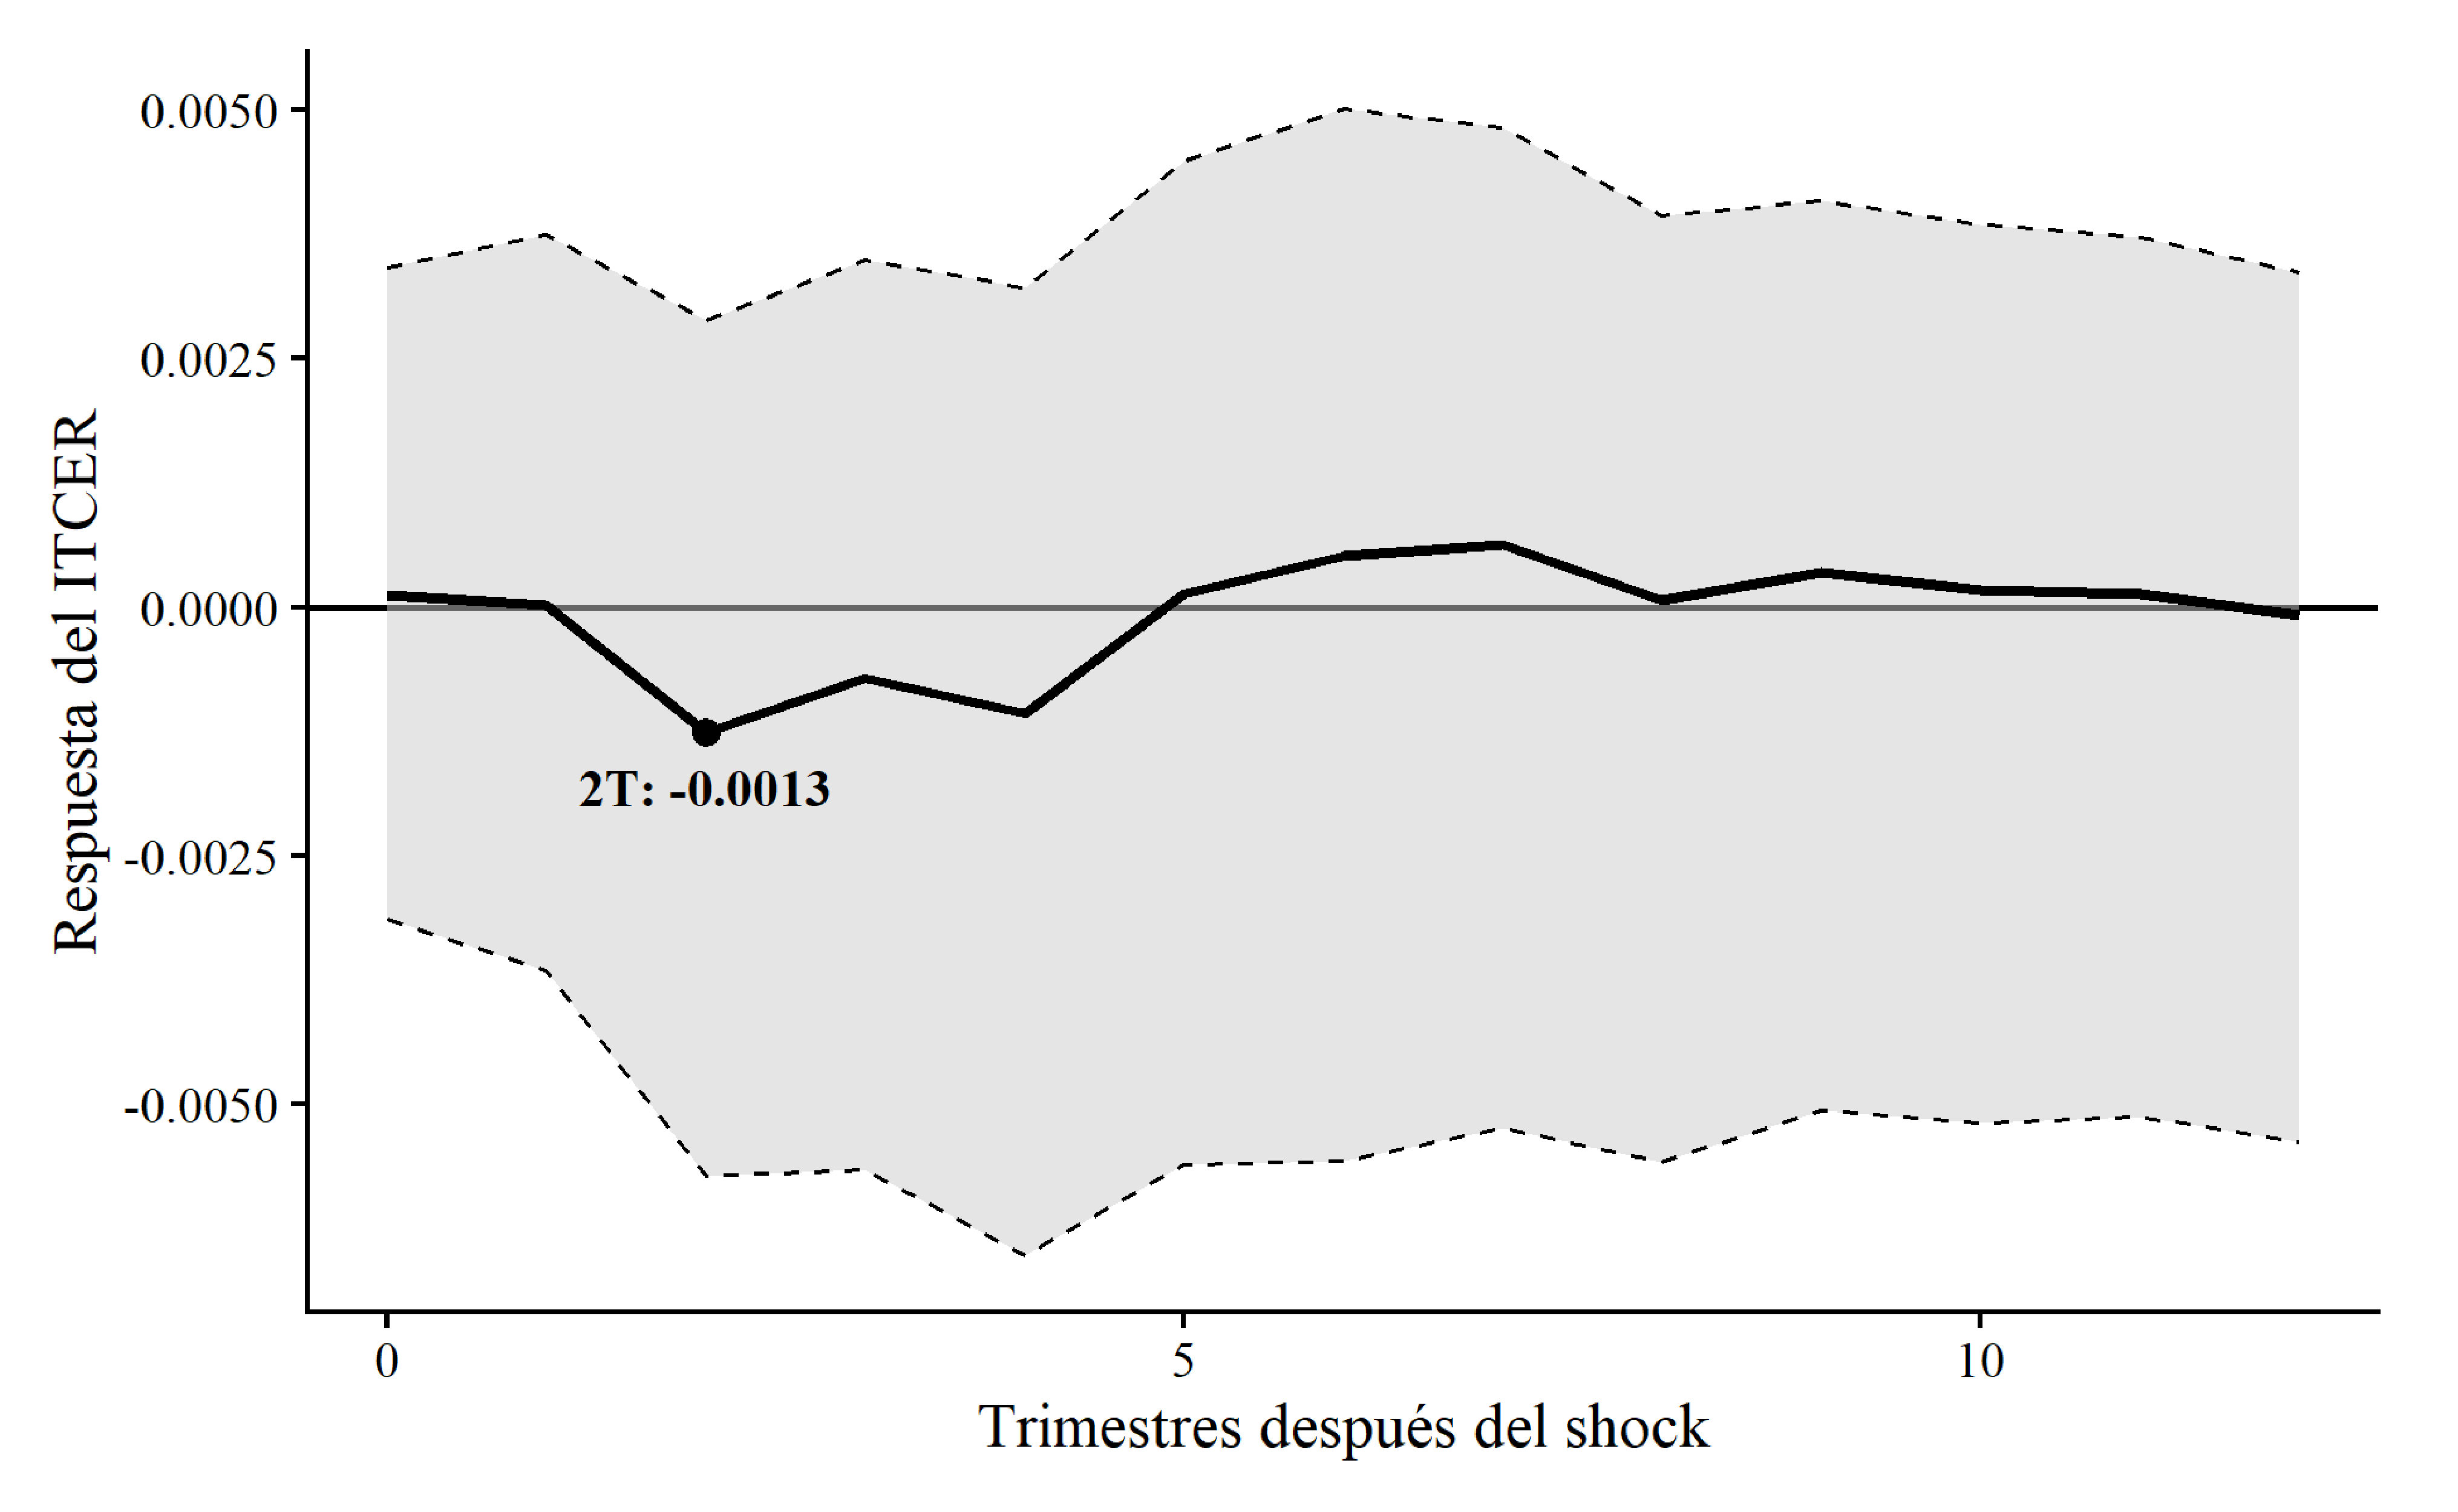
\includegraphics[width=0.8\linewidth]{../graficos/Impulso-Respuesta de la variable ITCER ante un choque estructural de Remesas (primer orden).pdf}

\vspace{-0.2cm}

\{\tiny Ausencia de Apreciación (Efecto Gasto nulo)\}
\end{column}

\begin{column}{0.5\linewidth}
\centering

\scriptsize IRF: Respuesta del Sector Transable ante Remesas

\vspace{0.1cm}

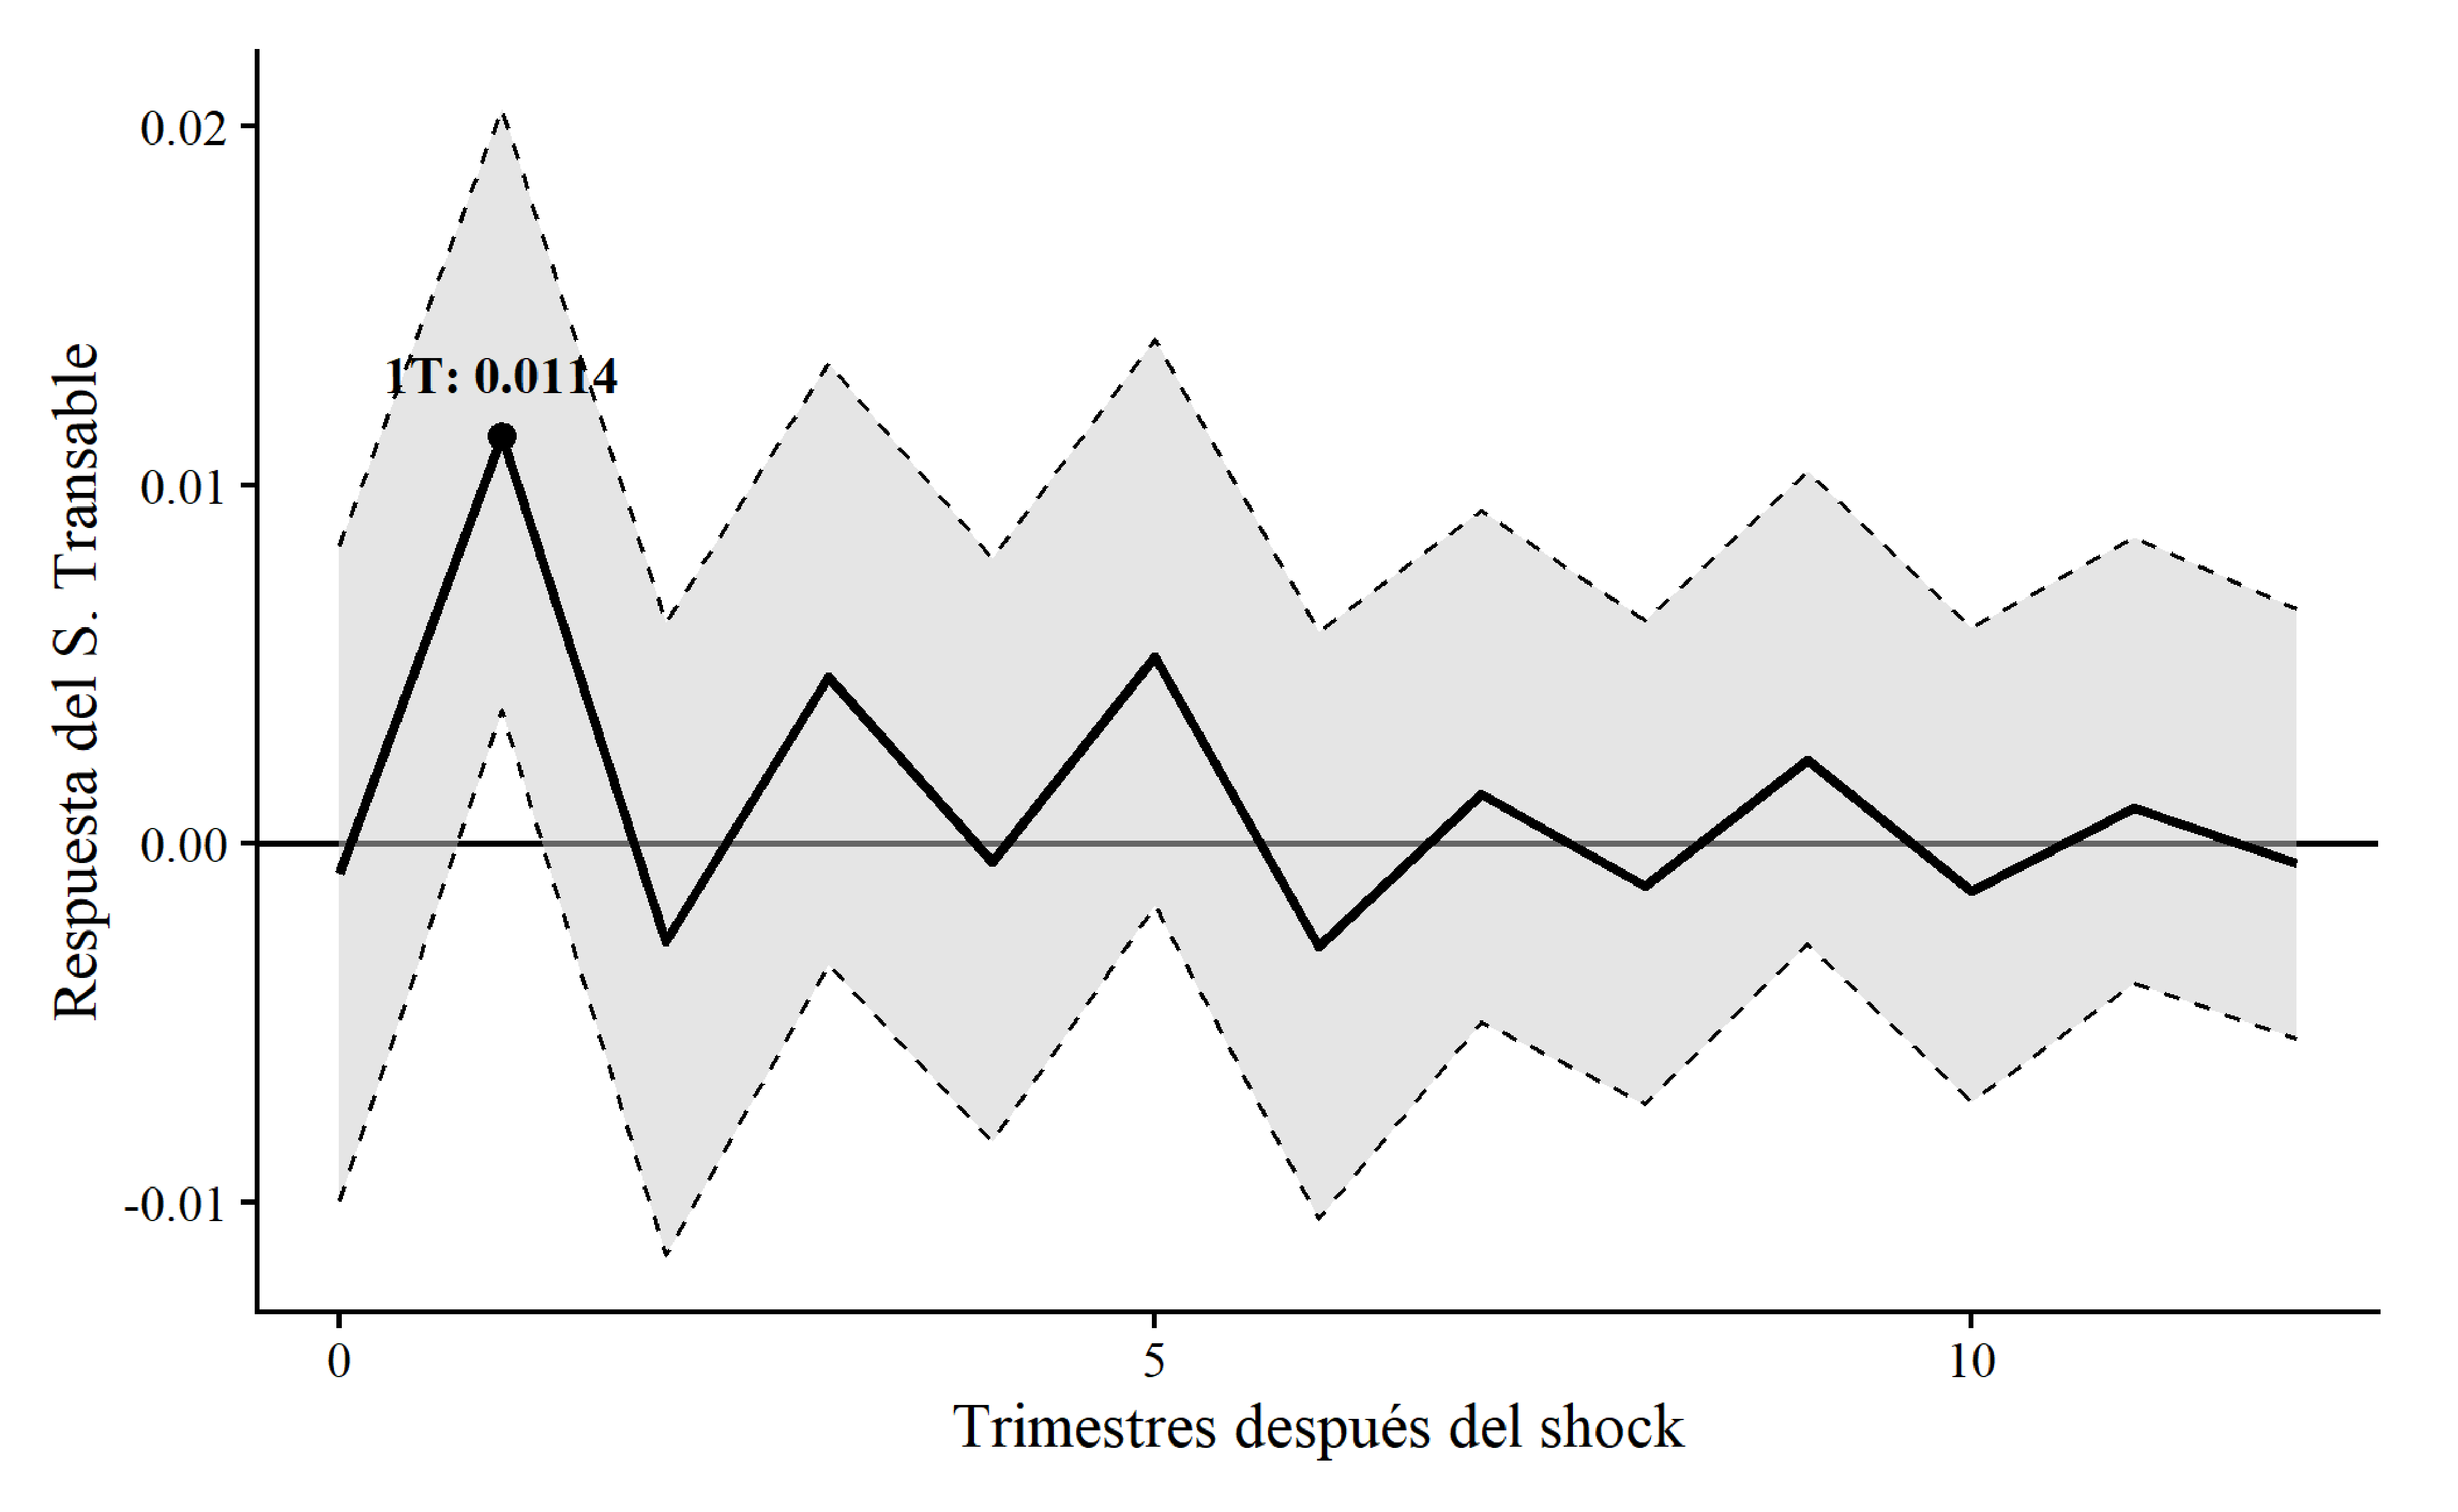
\includegraphics[width=0.8\linewidth]{../graficos/Impulso-Respuesta de la variable ST ante un choque de las Remesas (primer orden).pdf}

\vspace{-0.2cm}

\{\tiny Expansión del ST (Efecto Liquidez)\}
\end{column}
\end{columns}

\vspace{0.1cm}

\begin{itemize}
\tightlist
\item
  \textbf{Neutralidad Cambiaria:} El choque de remesas no altera los
  precios relativos. El intervalo bayesiano al 95\% contiene el cero a
  lo largo de los 12 trimestres.
\item
  \textbf{Sustituto de Crédito:} Respuesta expansiva transitoria y
  estadísticamente significativa en el Sector Transable (mediana de
  1.14\% en t=1).
\end{itemize}
\end{frame}

\begin{frame}{Impulso-Respuesta: Segundo Orden (Análisis de
Sensibilidad)}
\protect\phantomsection\label{impulso-respuesta-segundo-orden-anuxe1lisis-de-sensibilidad}
\begin{columns}[T]
\begin{column}{0.5\linewidth}
\centering

\scriptsize IRF: Respuesta del ITCER ante un choque de Remesas

\vspace{0.1cm}

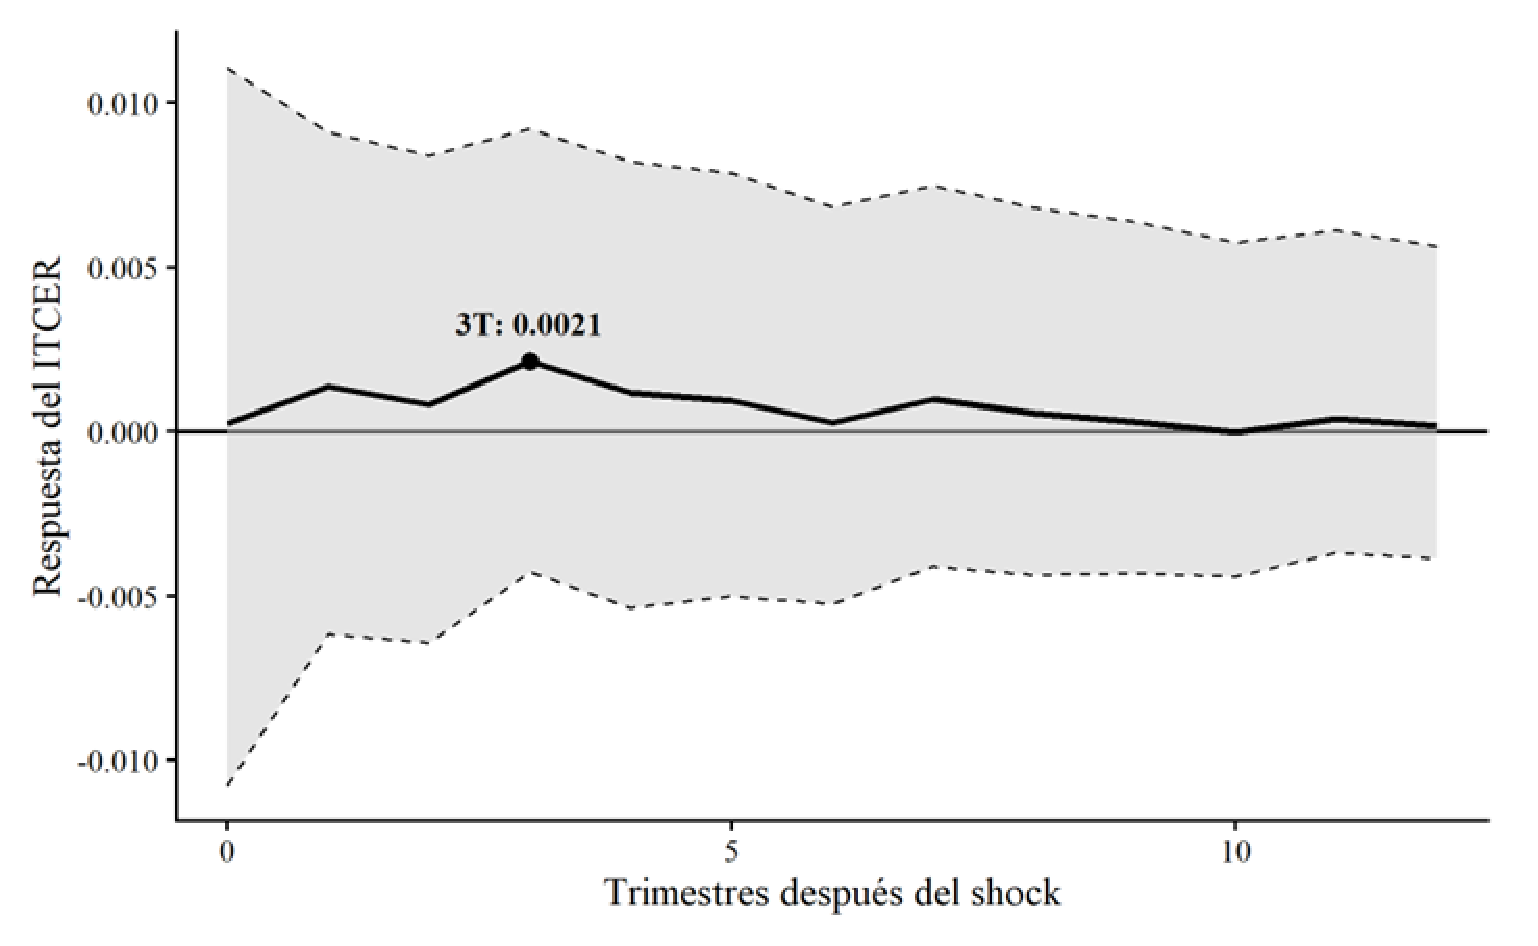
\includegraphics[width=0.8\linewidth]{../graficos/Impulso-Respuesta de la variable ITCER ante un choque de las Remesas (segundo orden).pdf}

\vspace{-0.2cm}

\{\tiny Invarianza del ITCER ante Remesas\}
\end{column}

\begin{column}{0.5\linewidth}
\centering

\scriptsize IRF: Respuesta del Sector Transable ante el ITCER

\vspace{0.1cm}

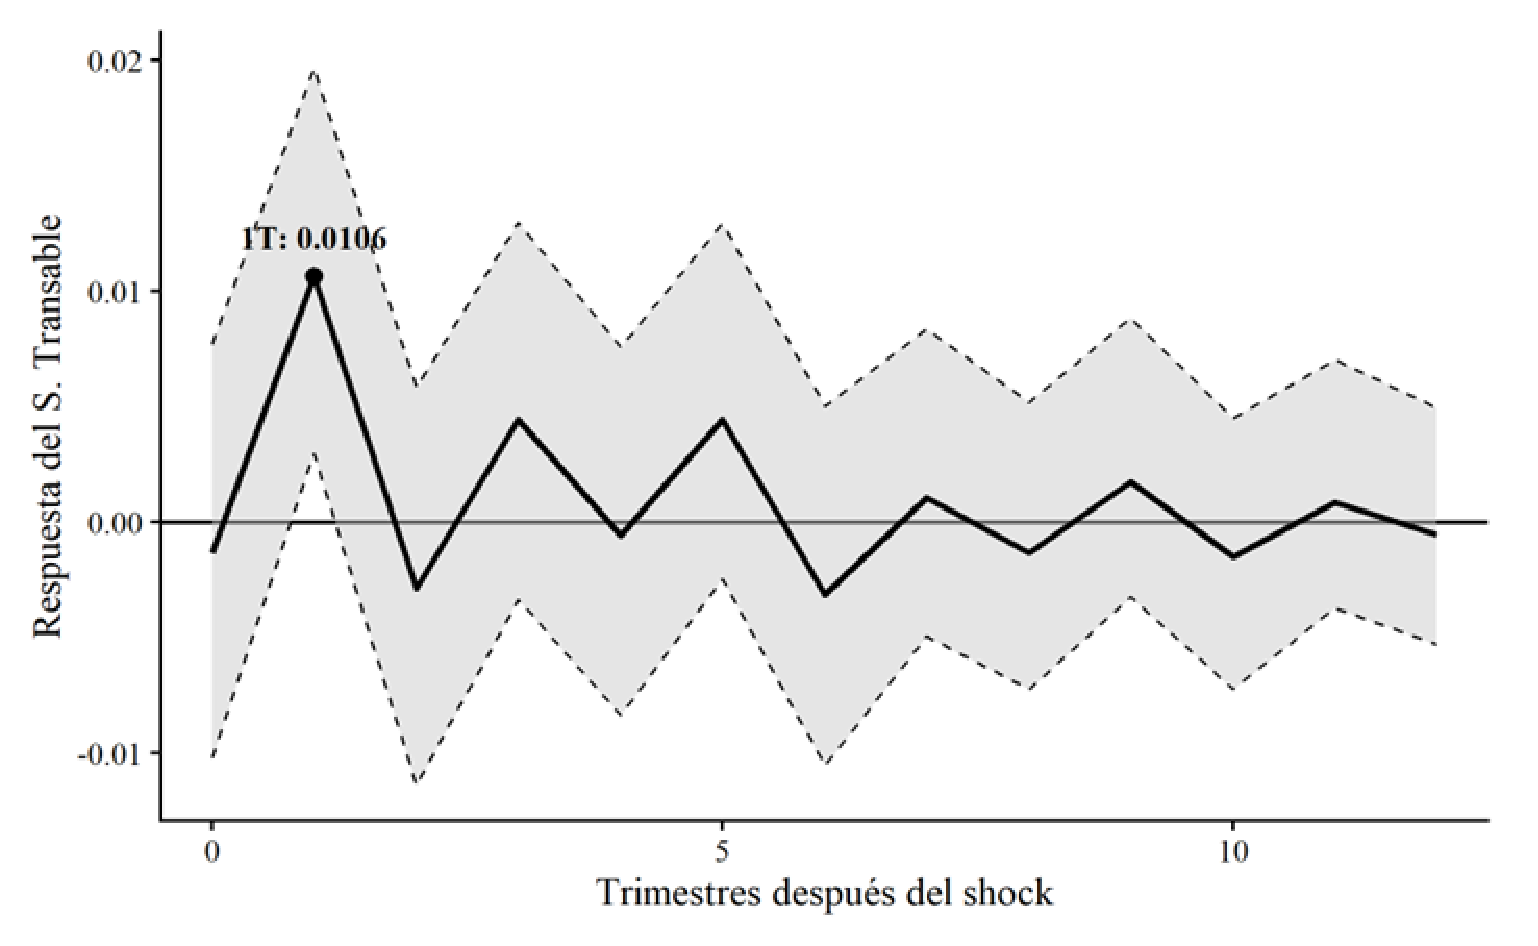
\includegraphics[width=0.8\linewidth]{../graficos/Impulso-Respuesta de la variable ST ante un choque del ITCER (segundo orden).pdf}

\vspace{-0.2cm}

\{\tiny Sensibilidad del ST ante el ITCER\}
\end{column}
\end{columns}

\vspace{0.1cm}

\begin{itemize}
\tightlist
\item
  \textbf{Robustez del Rechazo:} Al otorgar precedencia contemporánea al
  ITCER, el impacto de las remesas sobre el tipo de cambio sigue siendo
  nulo.
\item
  \textbf{Cadena Causal Rota:} Aunque el Sector Transable responde
  positivamente a ganancias cambiarias, las remesas son incapaces de
  provocar dicha alteración.
\end{itemize}
\end{frame}

\begin{frame}{Mecanismos de Transmisión Institucional}
\protect\phantomsection\label{mecanismos-de-transmisiuxf3n-institucional}
\begin{block}{¿Por qué no se materializa la Enfermedad Holandesa?}
\protect\phantomsection\label{por-quuxe9-no-se-materializa-la-enfermedad-holandesa}
La patología macroeconómica se encuentra desactivada desde su origen
debido a las restricciones institucionales y estructurales de la
economía nicaragüense:
\end{block}

\vspace{0.3cm}

\begin{enumerate}
\tightlist
\item
  \textbf{Válvula de Importaciones:} La altísima propensión marginal a
  importar drena rápidamente el exceso de divisas hacia el exterior,
  evitando que la liquidez presione los precios de los bienes no
  transables locales.
\item
  \textbf{Régimen Cambiario Administrado:} El \emph{crawling peg} actúa
  como ancla, esterilizando las presiones de apreciación nominal que
  exige el modelo clásico de Corden y Neary.
\end{enumerate}
\end{frame}

\begin{frame}{Discusión y Robustez}
\protect\phantomsection\label{discusiuxf3n-y-robustez}
\begin{block}{}
\protect\phantomsection\label{section}
\begin{itemize}
\tightlist
\item
  \textbf{Superación del enfoque BVAR tradicional:} El BVAR en
  diferencias omitía las relaciones de baja frecuencia y presentaba
  heterocedasticidad. El \textbf{BVECM} modela correctamente la
  cointegración y absorbe quiebres estructurales.
\item
  \textbf{Agenda Futura:} Explorar efectos asimétricos o no lineales
  mediante modelos de umbral (\emph{Threshold VAR}) debido a la escala
  histórica actual de los flujos.
\end{itemize}
\end{block}
\end{frame}

\begin{frame}{Conclusiones}
\protect\phantomsection\label{conclusiones}
\begin{itemize}
\tightlist
\item
  \textbf{Diagnóstico Final:} La hipótesis de la \textbf{Enfermedad
  Holandesa no se materializa} en la economía nicaragüense durante el
  periodo 2006--2023.
\item
  \textbf{Ausencia de Efecto Gasto:} El ITCER permanece inalterado
  debido a válvulas de escape estructurales (importaciones y régimen
  cambiario).
\item
  \textbf{Presencia de Efecto Liquidez:} Las remesas funcionan como un
  estabilizador macroeconómico y catalizador productivo de corto plazo
  que mitiga las restricciones financieras del sector transable.
\item
  \textbf{Transparencia y Replicabilidad:} El código de estimación y los
  datos están disponibles públicamente.
\end{itemize}
\end{frame}




\end{document}
